\section{\label{sec:methods} Methods}


Binary black hole mergers are often called ``dark sirens'' due to their lack observable EM counterparts.
Though the detection of an EM counterpart can facilitate the determination of host galaxy and therefore result in a well-constrained measurement of $H_0$ \cite{GW170817_H0}, such detections are rare: at time of writing, GW170817 is the only neutron start merger detection with an identified EM counterpart \cite{GW170817_announce}.

As early as 1986 it was proposed that an array of multiple gravitational wave detectors could be used to estimate the distance to an event $d_L$ and bounds on sky location \cite{Schutz_1986}.
Gravitational waves originating from a binary black hole system during the inspiral phase of the merger can be used as dark sirens due to the fact that the individual black hole masses can be determined from the gravitational wave frequency.
The power radiating from the binary system is due to its orbital energy, and therefore the power radiating from the source can be determined purely from the gravitational wave frequency, without any knowledge of the luminosity distance.
The power detected is related to this emitted power through an inverse square law, and so the luminosity distance can be determined without the need for a cosmic distance ladder.
Gravitational waves therefore present a completely independent method by which we can determine distances to galaxies, provided we can determine the host galaxy for a given merger \cite{GW170814_DES,GW170817_H0,Nair_2018}.

Since we can estimate the sky location from which the signal was emitted along with the distance to the event, these estimates can then be used to produce a catalog of candidate host galaxies from existing sky surveys.
Based on the posterior distributions for these localizations, we use a method for measuring $H_0$ layed out by Nair et al. \cite{Nair_2018}.
It has been predicted that these methods can confine the Hubble constant within the decade \cite{Chen_2018}.
This technique was applied to the event GW170814 by collaborators from the LIGO and Virgo teams using results from the Dark Energy Survey of the southern sky \cite{GW170814_DES}.
We carry out a similar analysis on simulated data sets based on historic GW data and simple physical assumptions for the distribution of galaxies within clusters.

%\section{Data} \label{sec:develop}

Historic data is taken from merger catalogs from the second and third year of LIGO observations \cite{GWTC_2,GWTC_3}. Our analysis is only interested in the solid angle covered by sky localization ($\Omega$), distances obtained from the GW data ($d_L$), and their uncertainties, $\sigma_d$. We thus marginalize over all other parameters to obtain a three dimensional probability distribution containing only these parameters of interest. It vastly simplifies our analysis if we assume that the uncertainties on $d_L$ are Gaussian. However, posterior distributions from the LIGO papers contain differing upper and lower confidences. We take the half width on these posteriors as our Gaussian uncertainties.

After obtaining these marginalized probability distributions, we use historic data as a training set for Gaussian kernel density estimation. We then use the kernel estimation to sample simulated events which have the same underlying probability distribution as observations. The returned samples have a finite probability to be from unphysical regions, i.e. $d_L \leq 0$, $\Omega\leq 0$ or $\sigma_d > d_L$. To counteract this, we reject all samples which are outside of the extremal historic values or violate the $\sigma_d \leq d_L$ constraint. Many of the sampled events will have very large localization regions, which makes it inconvenient to use them for estimates of $H_0$. Since our goal is to produce an estimate of how many observations are required to produce estimates of $H_0$ we only perform further analysis on events that were well localized.

After producing simulated GW events we need to select a suitable sky catalog. These data are also simulated by randomly sampling a number of galaxy clusters which are assumed not to interact with one another. The total mass of the cluster is assumed to follow a Press-Schechter mass distribution\cite{Press_1974}. Peculiar motions (which affect the measured redshift $z$) and distance from the center of mass are sampled such that the Virial theorem is obeyed, but other important factors like the very high concentrations of dark matter within clusters are neglected. More details on cluster generation are given in appendix \ref{append_b}.
    
%\subsection{\label{Method} Methodology}

We start with a simple application of Bayes' theorem,
\begin{align}
    p(H_0|d_{GW}, d_C)&\propto p(d_{GW}, d_C|H_0)p(H_0)\nonumber\\
    &= p(d_{GW}|H_0)p(d_C|H_0)p(H_0).
\label{eq:bayes}
\end{align}
where $d_{GW}$ refers to the observed data from the gravitational wave detectors and $d_C$ refers to data from the known catalog of stars and their redshifts. We break this joint likelihood into a product of likelihoods since both experiments are statistically independent.

Since we are considering dark sirens without electromagnetic counterparts, we do not know the host galaxy in which the merger occurred. Thus we must marginalize over all possible galaxies within the volume of possible locations supplied by the GW data. Since the number of galaxies is discrete, this is expressed as a sum:

\begin{align}
    p(&d_{GW}, d_C|{z_j, \hat{\Omega}_j},H_0)  \propto  \nonumber\\
    &\sum_{i} w_i \int dV p(d_{GW}|d_L, \hat{\Omega}_{GW}) 
    p(d_C|{z_, \hat{\Omega}_j}) \nonumber\\
    & \delta_D (d_L - d_L(z_i, H_0)) \delta_D (\hat{\Omega}_{GW} - \hat{\Omega}_i).
    \label{eq:marginal_like}
\end{align}
In principle, we should apply a weight to each galaxy $w_i$ we include this in the expression below, but for simplicity we take $w_i=1$ for all galaxies within the volume of interest and $w_i=0$ for all galaxies outside. This same approximation has been used in previous analyses \cite{Chen_2018,GW170814_DES,Nair_2018}. To evaluate this integral we switch to spherical coordinates and work in redshift space as opposed to distance space. This results in a change of coordinates

\begin{equation}
dV \propto \frac{d^2 V}{d z_i d\hat{\Omega}_i} \frac{d z_i}{d r} d r d\hat{\Omega} \propto \frac{r^2(z_i)}{H(z_i)}
\end{equation}
where $H(z_i)$ is the Hubble parameter in redshift space,

\begin{equation}
H(z_i) = H_0^3 \left(\Omega_m (1+z)^3 + \Omega_\Lambda\right)
\end{equation}
where we have assumed a flat universe so $\omega_k = 0$. We will take $\omega_m = 0.3$ and $\omega_\Lambda = 0.7$ in keeping with Soares-Santos et al. We expect our catalog of galaxies to have very low uncertainty on sky location, so we take $p(d_C|z_i,\Omega)=p(d_C|z_i)\delta(\Omega - \Omega_i)$. Finally we can write the posterior distribution for $H_0$:

\begin{align}
     p&(H_0|d_{GW}, d_C)\propto p(H_0) \sum_i \frac{1}{Z_i} \nonumber\\
     &\times \int dz_i p\left(d_{GW}|d_L(z_i, H_0), \hat{\Omega_{i}}\right)p(d_C|z_i)\frac{r^2 (z_i)}{H(z_i)}
    \label{eq: finaleq}
\end{align}
where $d_L(z_i, H_0) = cz_i / H_0$ uses Hubble's law to express luminosity distance in terms of redshift and an assumed value for $H_0$. We assume that the errors on redshifts are Gaussian, in keeping with the analysis by Singer et al. \cite{Singer_2016}. Under this assumption,

\begin{align}
    p&\left(d_{GW}|d_L(z_i, H_0)\right)\propto \nonumber\\
    &\frac{p(\hat{\Omega})}{\sqrt{2\pi}\sigma(\hat{\Omega})} \exp\left(-\frac{(cz_i/H_0 - \hat{d}_{GW})^2}{2\sigma_{GW}^2}\right).
    \label{eq:GW_like}
\end{align}

\begin{figure}
    \centering
    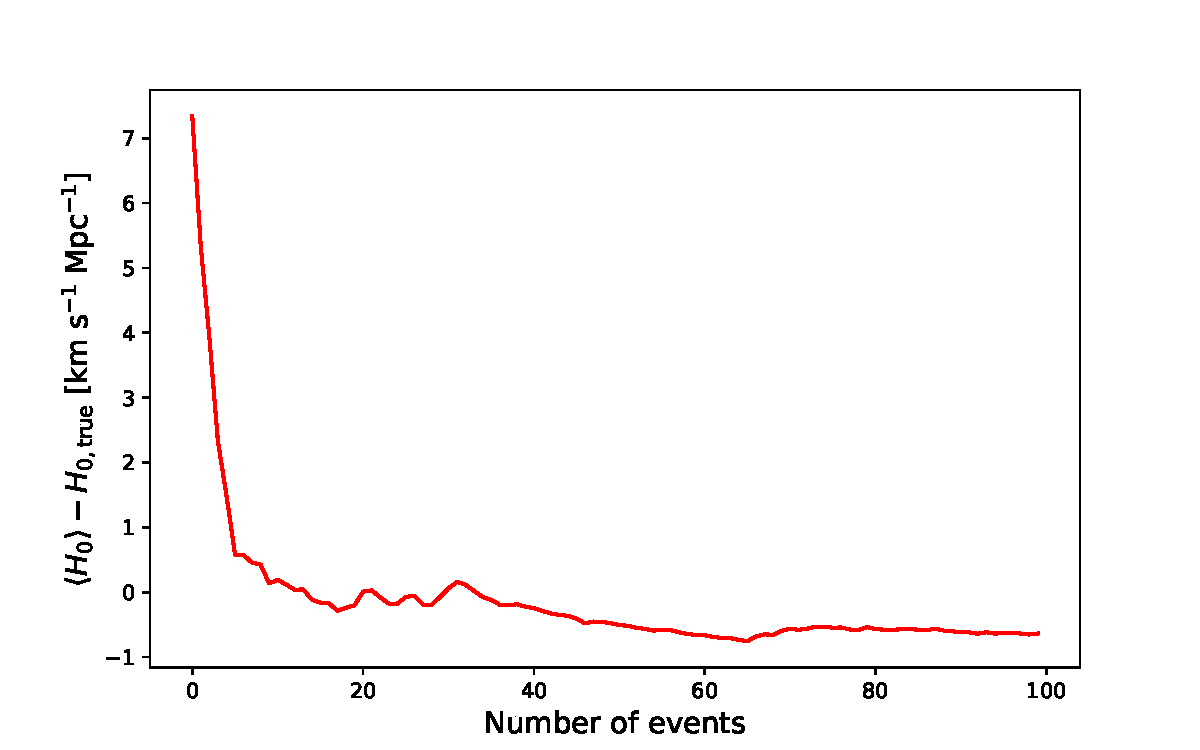
\includegraphics[width=\columnwidth]{figures/diff.pdf}
    \caption{The deviation between the injected known value of $H_0$ and our expectation value based on $p(H_0 | d_{GW}, d_C)$.}
    \label{fig:mean_diff}
\end{figure}

\begin{figure}
    \centering
    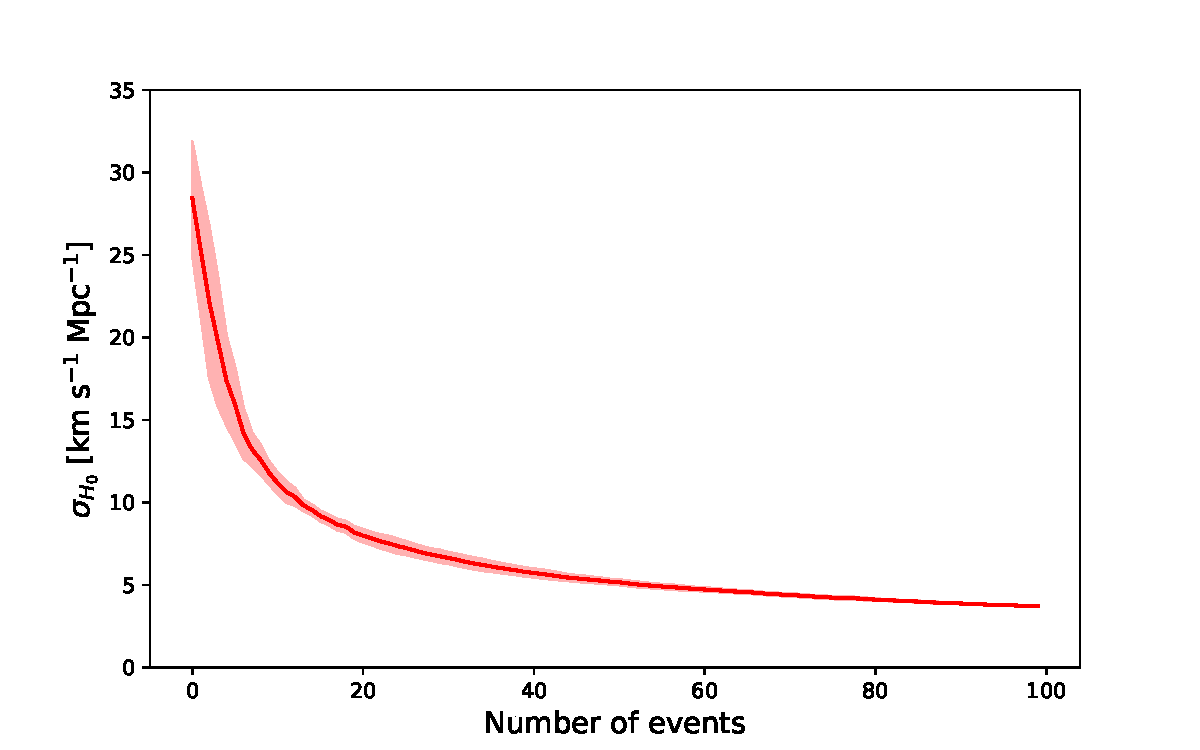
\includegraphics[width=\columnwidth]{figures/std.pdf}
    \caption{The standard deviation obtained from the posterior $p(H_0 | d_{GW}, d_C)$.}
    \label{fig:std}
\end{figure}

